\begin{frame}[fragile] \frametitle{Cello AMR: 1.~Patch Coalescing}
\centerline{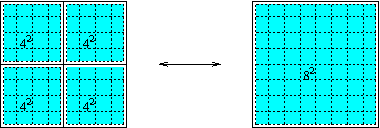
\includegraphics[width=2.5in]{coalesce.png}}
\begin{itemize}
\enhance{2}\item Coalesce patches into larger one when possible
\enhance{3}\item Split patches into smaller ones when necessary
\end{itemize}
\end{frame}

\begin{frame}[fragile] \frametitle{Cello AMR: 2.~Individual Child Refinement}
\centerline{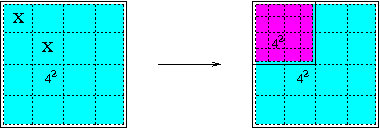
\includegraphics[width=2.5in]{amr-child.png}}
\begin{itemize}
\enhance{1}\item Refine children individually instead of all or nothing
\enhance{2}\item Added flexibility can reduce AMR tree size
\end{itemize}
\end{frame}

\begin{frame}[fragile] \frametitle{Cello AMR: 3.~Higher-order Refinement with Backfill}
\centerline{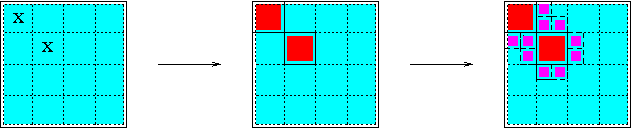
\includegraphics[width=3.5in]{kd-backfill.png}}
\begin{itemize}
\enhance{1}\item If $k=4$, refine by $4$ instead of $2$
\enhance{2}\item More ``targeted'' refinement
\enhance{3}\item Can optionally remove level jumps by ``backfilling'' levels
\enhance{4}\item Backfill patch locations known implicitly---nominal storage
\enhance{5}\item Many child nodes implies sparse storage
\end{itemize}
\end{frame}
